%%%%%%   TIPO DE DOCUMENTO: Reporte   %%%%%%
\documentclass[letterpaper,11pt]{report}
%%%%%%%%%%%%%%%%%%%%%%%%%%%%%%%%%%%%%%%%%%%%

%%%%%%%   PAQUETES   %%%%%%%
\usepackage[spanish]{babel} %Lenguaje: Espanol
\usepackage{graphicx} %Manejo de graficas e imagenes
%%%%%%%%%%%%%%%%%%%%%%%%%%%%

%%%%%%%   MARGENES DE PAGINA   %%%%%%%
\setlength{\oddsidemargin}{20pt} %20
\setlength{\topmargin}{1pt} %1
\setlength{\textheight}{22cm} %21
\setlength{\textwidth}{16.5cm} %16.5
%%%%%%%%%%%%%%%%%%%%%%%%%%%%%

\begin{document}

    %%%%%%% Renombrar en espaNol %%%%%%
    \renewcommand{\tablename}{Tabla} %Escribe Tabla en lugar de Cuadro
    \renewcommand{\listtablename}{\'Indice de tablas} %Escribe Indeice de tablas en lugar de Indice de cuadros

    %%%%%%%   PORTADA   y RESUMEN   %%%%%%%
    
\begin{center}
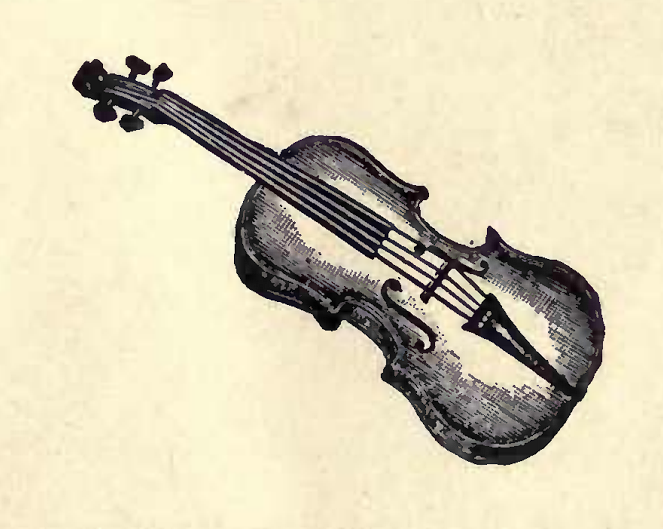
\includegraphics[width=0.5\textwidth]{../img/violin.png}
\end{center}

\begin{center}
\textbf{LOWELL, INDIANA.\\
Alfred Ha Miller}

\textbf{Copyright 1906,\\
Por Frederick Castle, M. D.\\
H. H. RAGON \& SON, Impresores,\\
Lowell, Indiana.\\
1906.}
\end{center}

\begin{center}
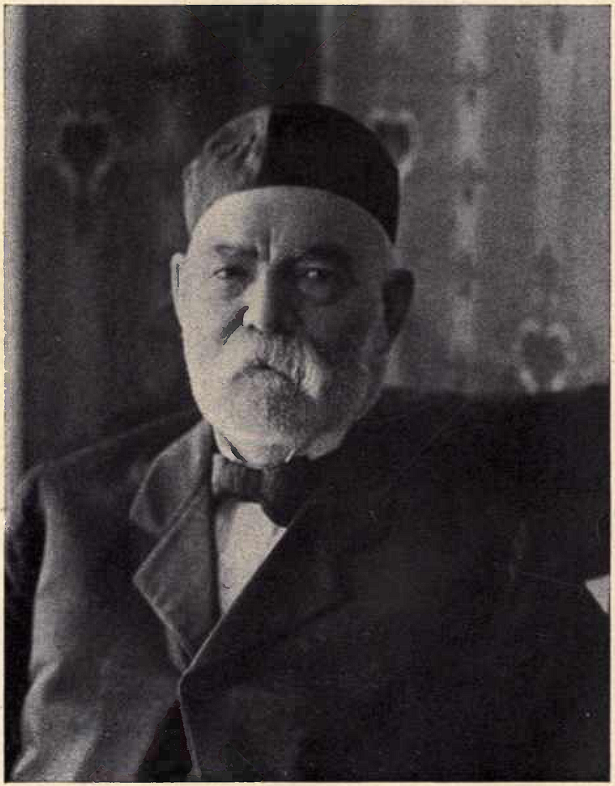
\includegraphics[width=1\textwidth]{../img/foto.png}
\par\smallskip
    \textbf{DR. FREDERICK CASTLE. }
\end{center} %incluye el archivo portada.tex
    %%%%%%%%%%%%%%%%%%%%%%%
%%%%    RESUMEN    %%%%
%%%%%%%%%%%%%%%%%%%%%%%

\begin{abstract}

  AquI va el resumen general del documento.

\end{abstract}
 %Incluir resumen del documento (resumen.tex)

    %%%%%%%   INCLUIR ENCABEZADOS EN INDICES Y CAPITULOS   %%%%%%%
    \pagestyle{headings}

    %%%%%%%   NUMERACION EN CONTENIDO E INDICE DE TABLAS Y FIGURAS   %%%%%%%
    \pagenumbering{roman} %NUmeros romanos
    %\setcounter{page}{1} %Comienza en I por default, aquI se puedo modificar

    %%%%%%   INCLUIR CONTENIDO, INDICE DE FIGURAS E INDICE DE TABLAS   %%%%%%
    \tableofcontents
    \listoffigures
    \listoftables

    %%%%%%%   NUMERACION EN CAPITULOS   %%%%%%%
    \clearpage %Para iniciar con los arAbigos
    \pagenumbering{arabic} %Numeros arabigos
    %\setcounter{page}{1} %Comienza en 1 por default, aquI se puede modificar

    %%%%%%%   INCLUYE CAPITULOS Y SECCIONES   %%%%%%%
    \chapter{T\'itulo del cap\'itulo 1} %CAP\'ITULO 1

    Contenido del cap\'itulo 1. %CapItulo 1 (capitulo1.tex)
	   \section{T\'itulo de la secci\'on 1}

Este es el contenido agregado de la secci\'on 1.

$criptoan\acute{a}lisis$ %SecciOn 1, inicia en otra pag. (seccion1.tex)
    % capitulo2.tex
\chapter{Marco Teórico}
Este es el segundo capítulo del documento.

\section{Antecedentes}
Contenido de los antecedentes.

\section{Estado del Arte}
Contenido del estado del arte. %CapItulo 2 (capitulo2.tex)
	   \section{T\'itulo de la secci\'on 1}

Este es el contenido agregado de la secci\'on 1.

$criptoan\acute{a}lisis$ %SecciOn 1, inicia en otra pag. (seccion1.tex)
	   
\end{document}
